\label{section:foreign_relations_supervised_model}

\begin{figure}
  \center
  \vspace{-55pt}
  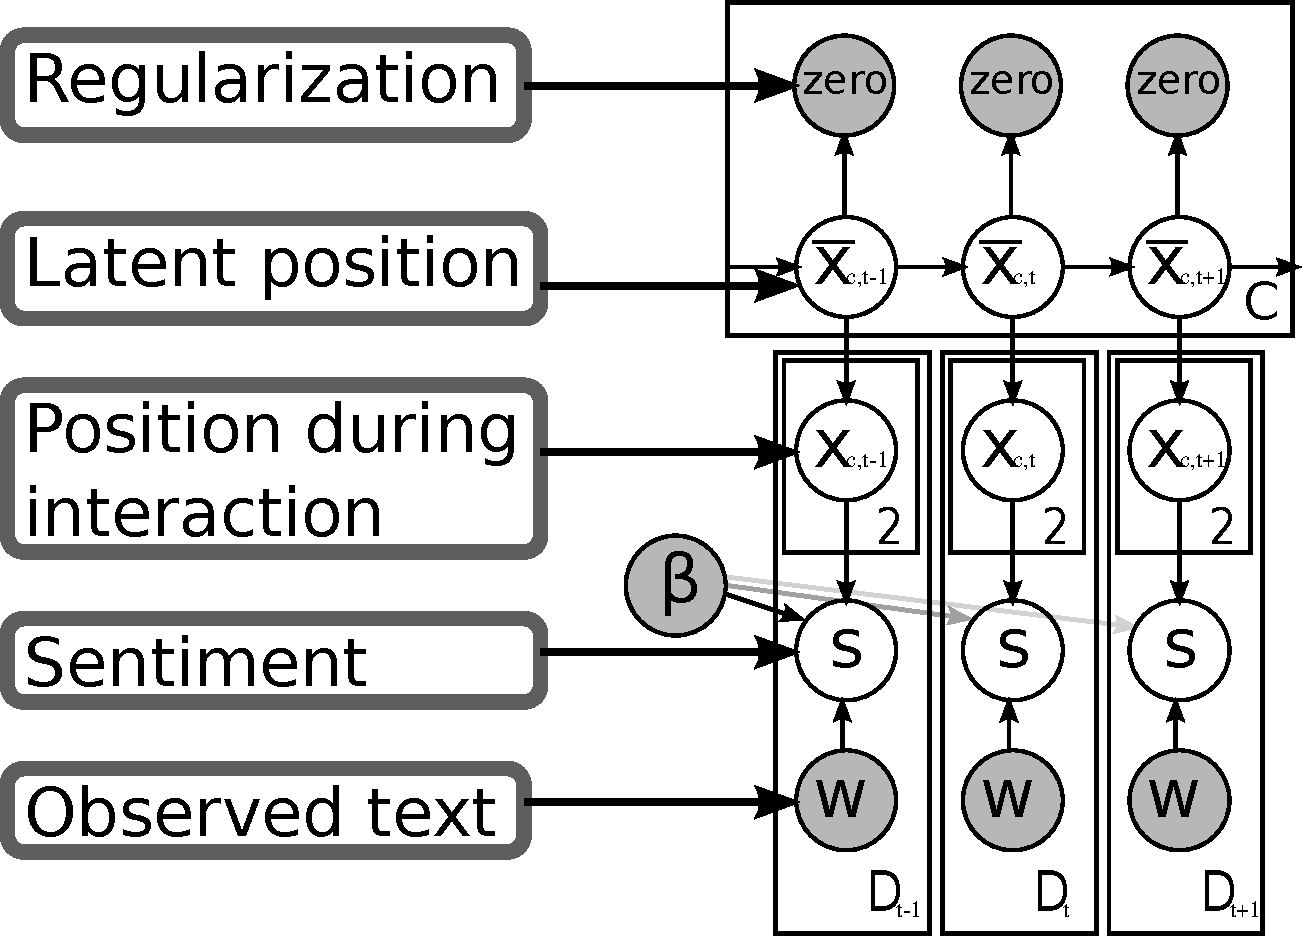
\includegraphics[width=0.5\textwidth]{chapter_foreign_relations/figures/countries_gm.pdf}
  \caption{A time-series model of countries' interactions.
    Pseudo-observations of ``zero'' are added for regularization.
    Amazon Mechanical Turk labels are used to fit $\beta$, which is
    used to infer unobserved sentiments.}
  \label{figure:gm}
\end{figure}
Reflecting the intuitions above, we assume that each nation lies in a
space of latent `''foreign sentiment''.  A spatial a model has two
benefits. First, it provides interpretability: nations with similar
positions in this latent space tend to interact more positively, while
nations further apart tend to have more tension in their relationship.
A spatial model also allows us to draw on ideas from
multidimensional scaling, which has been used successfully in both
political science \cite{martin:2002,jackman:2001} and social network
modeling \cite{hoff:2002,chang:2009}.

In the model we outline below, we assume that each country $c$ takes a
position $\bar x_c \in \mathcal{R}^P$ in the space of latent political
sentiment. The relationship between two countries will be determined
by the interaction of their positions $\bar x_c$.

\subsection{Related work}
% Covariates of war
% united nations general assembly

\paragraph{A temporal model of interaction.}
Foreign relations are not static, however; nations' alliances and
preferences change over time with the evolution of economies,
technology, and culture.  We make a further assumption that each piece
of news $d$ about two nations $c_1$ and $c_2$ reflects some underlying
sentiment $s_d$ between them.  We make this a fully temporal model by
allowing each country's mean position $\bar x_{c,t}$ to drift over
time with the Markov transition
\begin{align}
  \bar x_{ct} | \bar x_{c,t-1} \sim N(\bar x_{c,t-1}, \sigma_K^2),
\end{align}
as shown in Figure~\ref{figure:gm}. At any time $t$, state $c_1$ may interact with state $c_2$ in the following way:
\begin{align}
  x_{c_1,d} \sim N(\bar x_{c_1, t}, \sigma_D^2) \nonumber \\
  x_{c_2,d} \sim N(\bar x_{c_2, t}, \sigma_D^2) \nonumber \\
  s_d := x_{c_1,d}^T x_{c_2,d}, \nonumber \\
\label{equation:sentiment}
\end{align}
where we interpret $s_d$ as the sentiment between $c_1$ and $c_2$ as
reflected by article $d$.  When $c_1$ and $c_2$ are similar (as
measured by their inner product), their sentiment $s_d$ will be
positive; if they are dissimilar, their sentiment will be negative.
More extreme values indicate stronger sentiment.


\label{section:text_regression}
When a news source discusses the relationship between these nations,
the author's choice of words $\bm w_d$ reflects the relationship
between the countries.  We model this sentiment with the text of the
article $d$.  Using text regression \cite{kogan:2009}, the sentiment is modeled on wordcounts $\bm w_d$ of the article:
\[
  s_d | \bm w_d, \beta \sim \mathcal{N}( \bm w_d^T \beta , \sigma_W^2 ).
\]
We describe how to fit $\beta$ with Amazon Mechanical Turk workers in
Section~\ref{section:mturk}.

% In addition, a UN resolution may come up for vote at any time.  States
% cast a vote based on their current positions:
% \begin{align}
% x_{c_1,d} \sim N(\bar x_{c_1, t}, \sigma_D^2) \nonumber \\
% p(v_{cr}) = \sigma(x_{c_2, t} b_r + a_r) \nonumber \\
% \end{align}

% \begin{wrapfigure}{r}{0.4\textwidth}
%   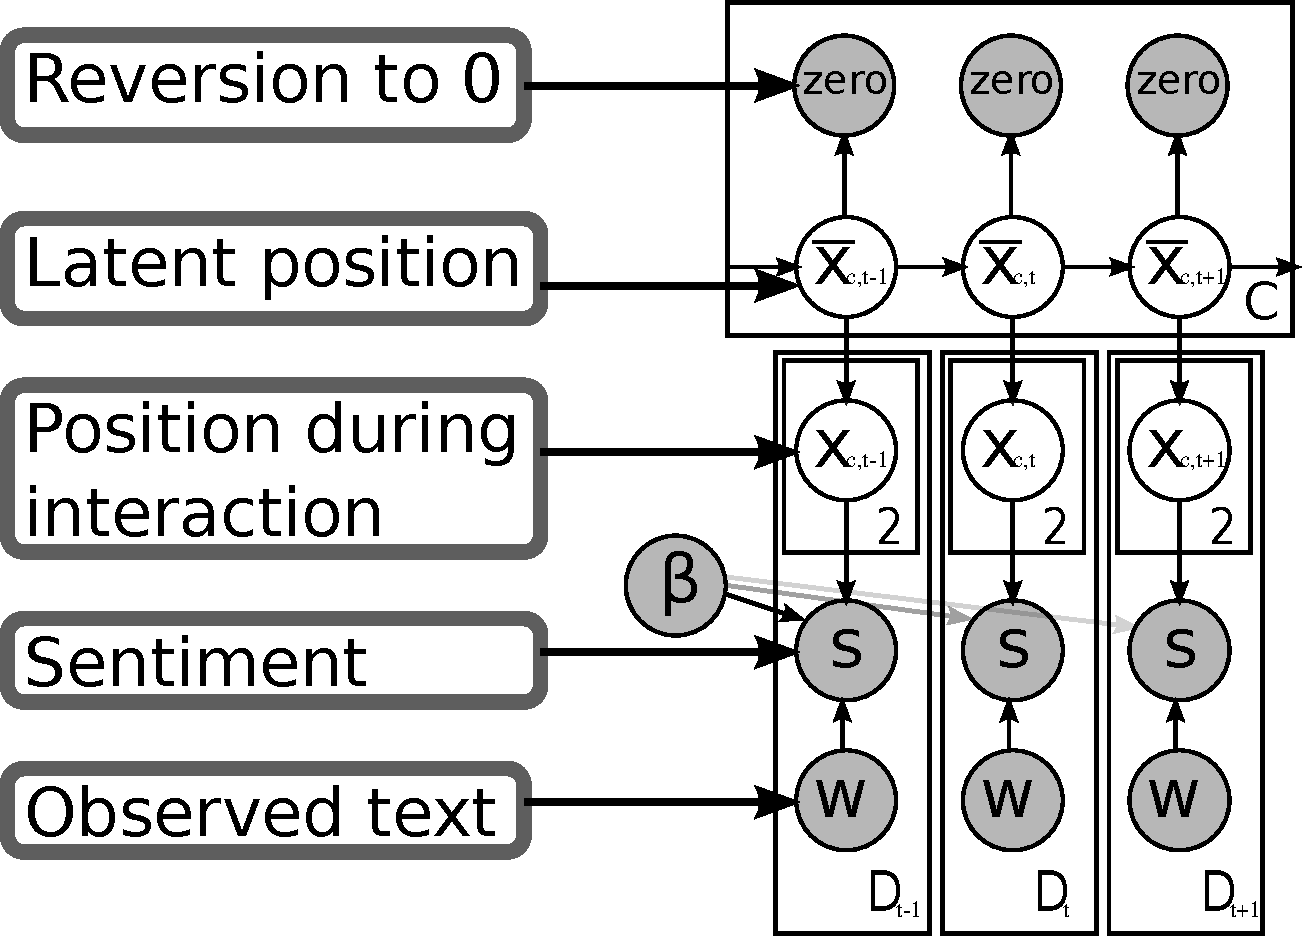
\includegraphics[width=0.4\textwidth]{figs/countries_gm.pdf}
%   \caption{The full time-series model of interaction by countries.
%     The large plate shows replication of a Markov chain for each
%     country.  Certain countries interact at each epoch -- possibly
%     multiple times -- with sentiment $s$.}
%   \label{fig:countries_by_ip}
% \end{wrapfigure}

\subsection{Related work}

% Democracy, Political Similarity, and International Alliances, 1816-1992
% Brian Lai
% Dan Reiterb
% Department of Political Science, Emory University
Spatial models such as Item Response Theory (IRT) have been developed
over the past century by quantitative social scientists for analyzing
behavior.  While much of this work has been used to model
parliamentary voting behavior, these techniques have also been used to
model voting in the UN General Assembly. Gartzke et al., for example,
use these votes and alliance models to study the nations' affinities
\cite{gartzke:1998}.

These models have been developed for dyadic data more fully in network
models such as the latent space model \cite{hoff:2002,sarkar:2005}, in
which the probability of a link between two nodes is a function of
their latent-space distance.  The qualitative relationship of
entities' dyadic relationships has been more fully developed with text
by the relational topic model, which uses free text to model the
relationship between actors in an unsupervised setting
\cite{chang:2009}.
% Supervised topic models


% Affinity of states dataset: 
% Fading Friendships (working paper)
% Alliances, Affinities and the Activation of International Identities∗
% Erik Gartzke†
% Alex Weisiger‡
% 7 March 2011

\section{Inference}
We fit the \emph{MAP} objective of this probabilistic model.  This has
the benefit of both clean exposition and simple implementation, and it
can be interpreted as a form of unregularized variational inference.
We optimize the \emph{MAP} objective in this model using traditional
EM.

\paragraph{M Step.} In the M step, the mean of each country's position
is updated using a modified Kalman filter.  This step differs from a
standard Kalman filter in that we may have no or multiple observations
on any given date.  We also add \emph{pseudo-observations} for each
country at each day $t$ with mean 0 and variance 10.  These
observations are a form of ``time-series regularization'' and reflect
the sense that a lack of news is effectively neutral news. The prior
over the ends of the chain are standard normal.

\paragraph{E Step.} In the E-step, our goal is to infer nations'
positions $x_{c,d} | \bar{x}_{c,t_d}, s_d$ with each interaction $d$ given
their means and the sentiment $s_d$ for this interaction.  We find
these positions by gradient ascent on $x_{c,d}$.

\section{Estimation of sentiment $s$}
\label{section:sentiment_models}
To infer the sentiment $s_d$ between two countries, we treat the
corresponding news article as a bag-of-words and use text regression
\cite{kogan:2009}.  In each of these cases, the sentiment $s_d$ is
first estimated on a training set using Amazon Mechanical Turk (AMT).
AMT is a crowdsourcing platform which provides access to thousands of
``workers'' who perform simple tasks over the Internet.  These labels
are then attached to all articles by predicting their sentiment.

\section{Empirical studies: comparisons with ground truth}

\label{section:experiments}

We fit and evaluate this model over news articles discussing 245
nations from twenty years of the \emph{New York Times} (NYT).  This
collection spanned the years 1987 to 2007, a period which included
both Gulf wars; the collapse of the Soviet Union; the reunification of
Germany; September 11th, 2001; and countless other world events.

\subsection{Datasets and tokenization}  We made an important
assumption that the scope of foreign sentiment discussion is at the
level of a paragraph.  We therefore used the subset of paragraphs
which discuss exactly two nations as ``documents'' $d$, a set of
257,472 distinct paragraphs which came from the foreign, business,
financial, and magazine desks of the newspaper during this period. We
used standard stopword filters and removed the geographic tags for
labeling nations from the sentiment vocabulary.

\subsection{Human labels with Amazon Mechanical Turk}
\label{section:mturk}
\begin{figure*}
  \setlength\fboxsep{0pt}
  \setlength\fboxrule{0.5pt}
  \center \fbox{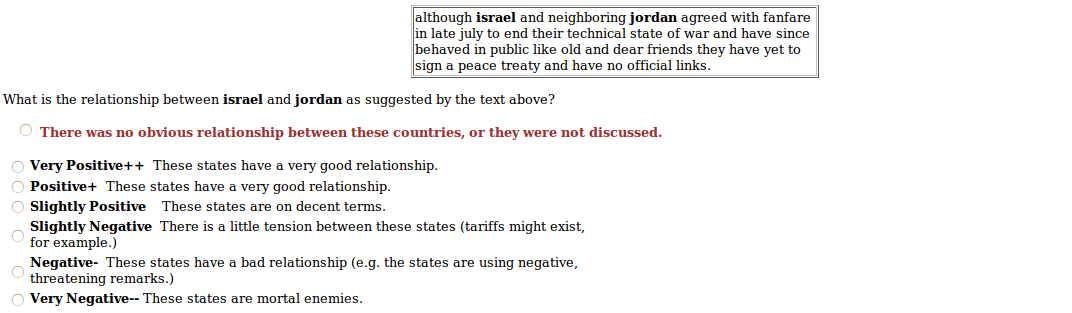
\includegraphics[width=1.0\textwidth]{chapter_foreign_relations/figures/mturk_screenshot.png}}
  \label{figure:mechanical_turk_sample}
  \small\caption{A screenshot of a Mechanical Turk labeling task.
    Sometimes relationships may be complicated; both raters gave this
    example a score of ``slightly positive''.}
  \normalsize
\end{figure*}

To fit the model, we asked \emph{Amazon Mechanical Turk} raters to rate the
sentiment between two nations mentioned in a paragraph in the range -5
= "mortal enemies'', $\ldots, 5 = $''very good relationship''.
With these training examples, we fit the coefficients $\beta$ of the
text regression discussed in Section~\ref{section:model}.  This
coefficient was then fixed in the joint model in
Figure~\ref{figure:gm} to allow us to learn sentiment from
paragraphs' words.  We trained and fit the model with the following procedure:

\begin{enumerate}
  \item Randomly select 3607 paragraphs discussing pairs of 245 countries.
  \item Label each of these paragraphs' sentiment with two ratings
    from Amazon Mechanical Turk.
  \item Hold out 42 random country pairs (244 paragraphs) for testing.
  \item Estimate sentiment model parameters $\beta$ using the training
    paragraphs.
  \item Infer the spatial sentiment model with these parameters on
    all 257,472 paragraphs.
  \item Evaluate model sentiment prediction on the heldout 244 test
    paragraphs.
\end{enumerate}
  
\subsection{Expert labels: Correlates of War}x

\subsection{Results}
 \begin{figure}
  \begin{tabular}{ccc}
    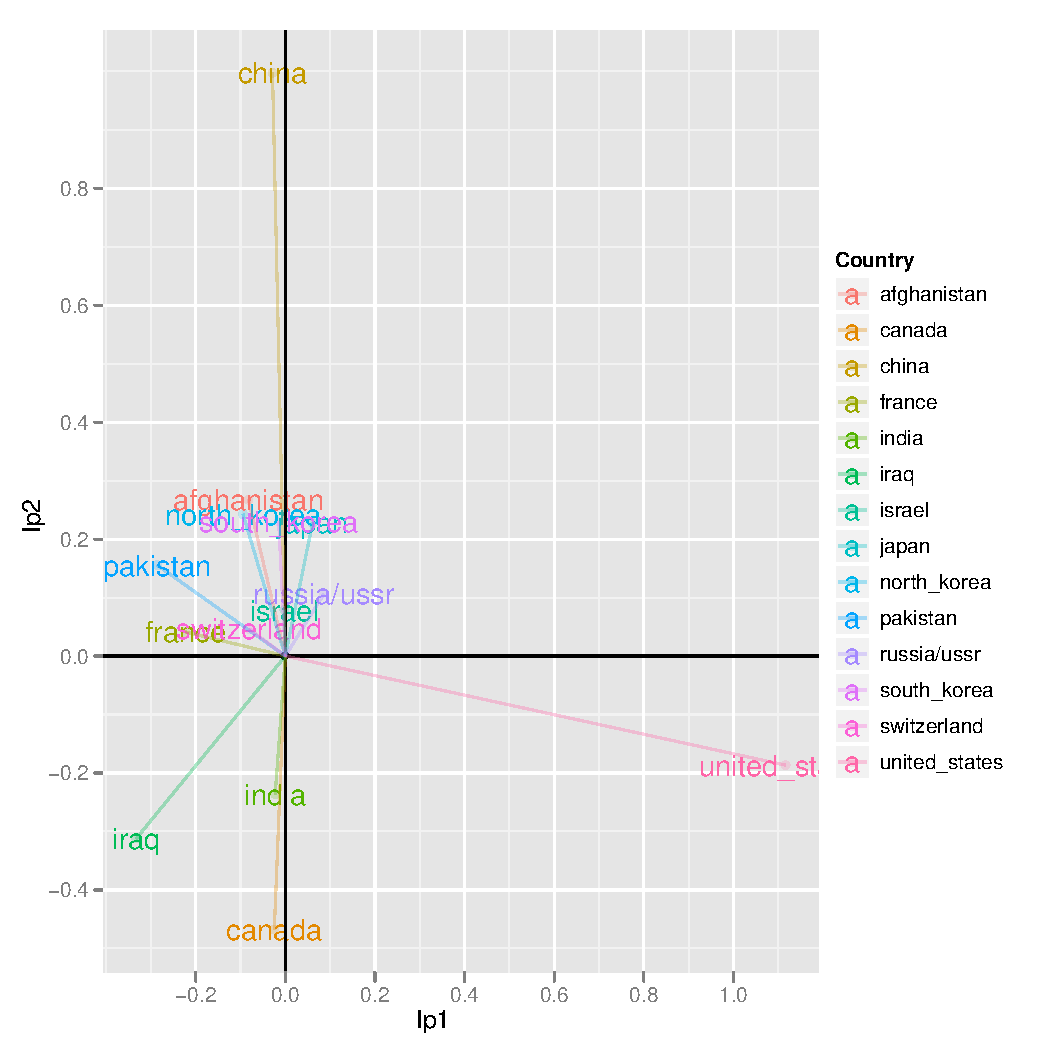
\includegraphics[width=0.33\textwidth]{chapter_foreign_relations/figures/002_countries_by_ip_1987.pdf} &
    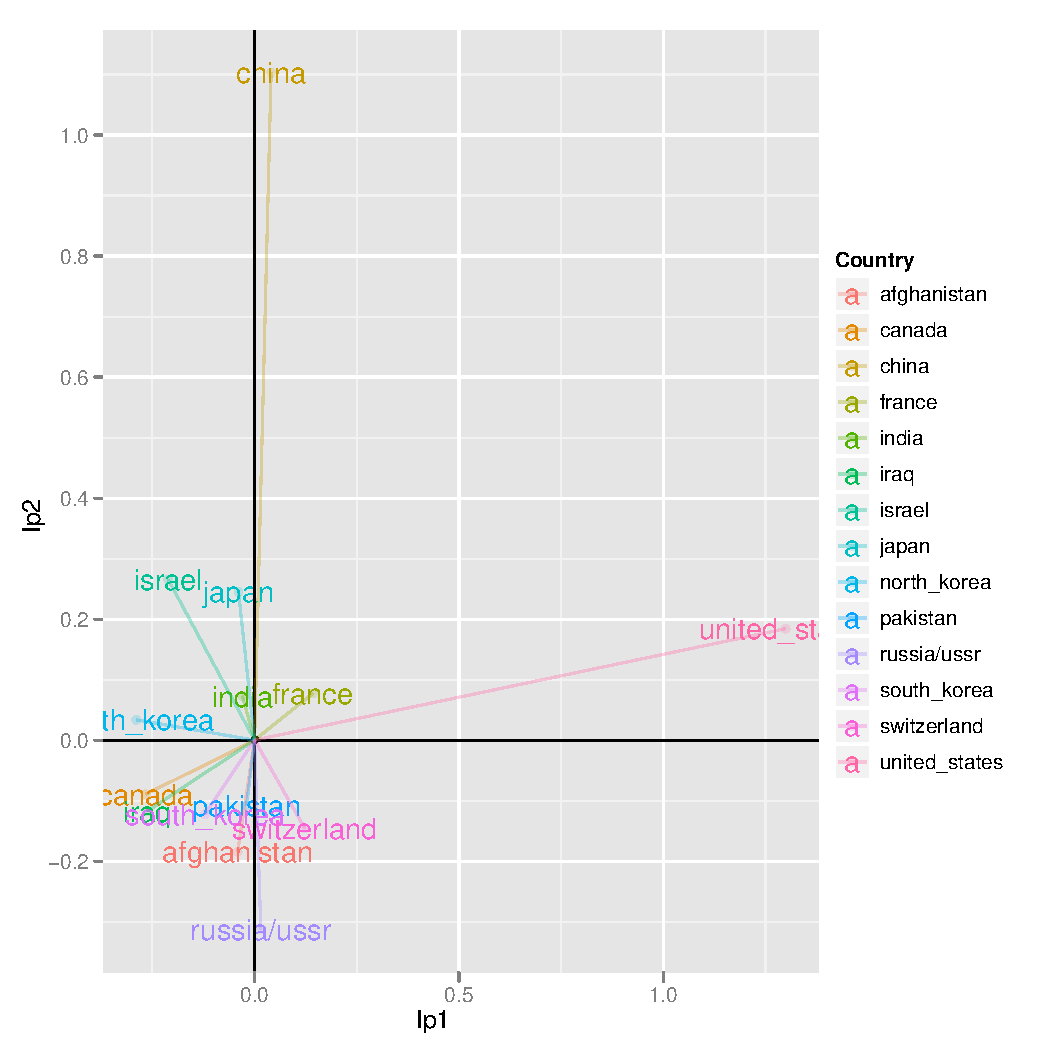
\includegraphics[width=0.33\textwidth]{chapter_foreign_relations/figures/002_countries_by_ip_2007.pdf} &
    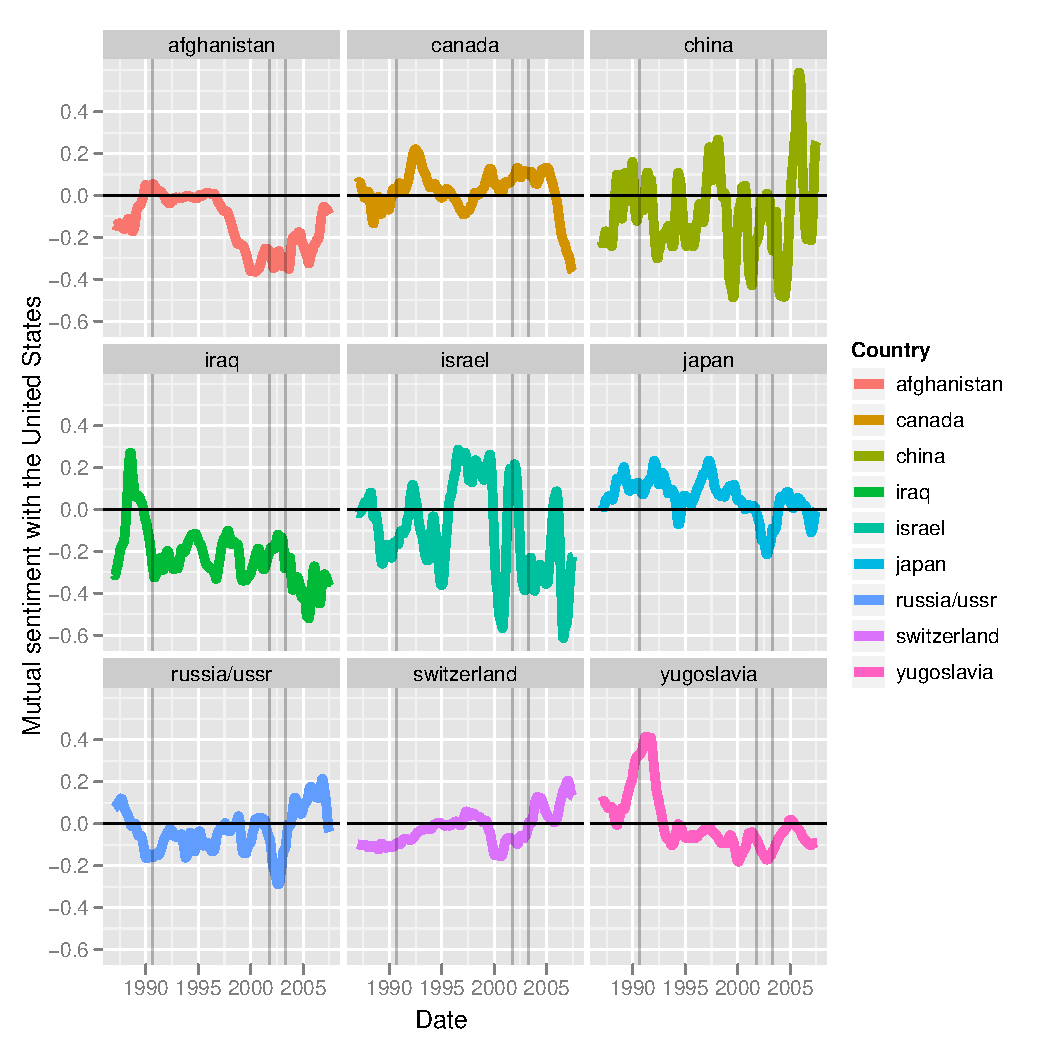
\includegraphics[width=0.33\textwidth]{chapter_foreign_relations/figures/002_us_vs_everyone.pdf} \\
    (a) & (b) & (c) \\
  \end{tabular}
  \caption{
    (a) Example positions of selected countries in the latent space of national sentiment, in 1987. Sentiment is given by the inner product between two vectors.
    (b) Example positions of selected countries in 2007.
    (c) Mutual sentiment $s = \bar x_{c, \cdot}^T \bar x_{\mbox{\small us}, \cdot}$ with the United States over time. The two Iraq wars and September 11th, 2001 are marked.
  }
  \label{figure:figures}
\end{figure}

\paragraph{Heldout sentiment}
 \begin{table}[t]
   \caption{Average error predicting sentiment $s_d$ between heldout nation pairs.}
   \begin{center}
   \begin{tabular}{|c|c|c|}
     \hline
     Model & Mean Squared Error & Mean Absolute Error \\
     \hline
     Inter-rater agreement & 1.77 (7.11) & 1.037 (2.07) \\
     \hline
     Text regression & 5.53 & 1.94 \\
     \hline
     Prior variance 0.1 & 2.36 & 1.09 \\
     Prior variance 1 & \textbf{2.32} & \textbf{1.07} \\
     Prior variance 10 & 2.32 & 1.08 \\
     Prior variance 100 & 2.34 & 1.09 \\
     Prior variance 1000 & 2.33 & 1.08 \\
     \hline
   \end{tabular}
   \label{figure:sse_test}
   \end{center}
\end{table}


\paragraph{Heldout sentiment}
 \begin{table}[t]
   \caption{Average error predicting sentiment $s_d$ between heldout nation pairs.}
   \begin{center}
   \begin{tabular}{|c|c|c|}
     \hline
     Model & Mean Squared Error & Mean Absolute Error \\
     \hline
     Inter-rater agreement & 1.77 (7.11) & 1.037 (2.07) \\
     \hline
     Text regression & 5.53 & 1.94 \\
     \hline
     1 & \textbf{2.33} & \textbf{1.08} \\
     2 & 2.37 & 1.09 \\
     3 & 2.36 & 1.09 \\
     4 & 2.38 & 1.09 \\
     5 & 2.40 & 1.10 \\
     6 & 2.38 & 1.10 \\
     7 & 2.40 & 1.10 \\
     \hline
   \end{tabular}
   \label{figure:sse_test}
   \end{center}
\end{table}

 \begin{table}[t]
   \caption{Average error predicting sentiment $s_d$ between heldout nation pairs for Correlates of War.}
   \begin{center}
   \begin{tabular}{|c|c|c|c|}
     \hline
     Dimension & & Mean Squared Error & Mean Absolute Error \\
     \hline
     Text regression & & 3.37 & 1.12 \\
     \hline
     Mean & & 3.68 & 1.19 \\
     \hline
     \hline
     Dimension & Reversion variance & Mean Squared Error & Mean Absolute Error \\
     \hline
     1 & 10 & 0.628 & 0.389 \\
     2 & 10 & 0.561 & 0.287 \\
     \textbf{3} & 10 & 0.559 & 0.286 \\
     4 & 10 & 0.562 & 0.308 \\
     5 & 10 & 0.557 & 0.306 \\
     6 & 10 & 0.535 & 0.142 \\
     7 & 10 & 0.535 & 0.140 \\
     \hline
     3 & 0.1 & 0.539 & 0.163 \\
     3 & 1 & 0.555 & 0.245 \\
     3 & \textbf{10} & 0.559 & 0.286 \\
     3 & 100 & 0.560 & 0.296 \\
     3 & 1000 & 0.561 & 0.298 \\
     3 & 10000 & 0.561 & 0.298 \\
     \hline
   \end{tabular}
   \label{figure:sse_test}
   \end{center}
\end{table}

For two nations $c_1$ and $c_2$ mentioned together at time $t$, we
predict their sentiment to be $\tilde s_{c_1, c_2} = \bar x_{c_1,t}
\bar x_{c_2, t}$.  Based on this estimate, the average squared error
for heldout nations is 2.32 ($R^2=0.51$), considerably better than a
baseline of text regression, which had means-squared-error $5.53$; for
comparison, average \emph{inter-rater squared error} -- the minimum
theoretically possible given the set of Mechanical Turk ratings -- was
$1.77$, and the square of the difference \emph{between} raters was
$7.11$.  We also found that using ``pseudo observations'' with even
modest observation variance improves predictive performance; these
results are summarized in Table~\ref{figure:sse_test}.

Nations' positions are illustrated in Figure~\ref{figure:figures}.
Figures~\ref{figure:figures}(a,b) show nations' relative positions
and interactions for a two- dimensional model; heldout error slightly
increased for higher dimensions. The United States' relationship with
Iraq (see Figure~\ref{figure:figures}(c)) serves as an excellent
example of this model in action; the relationship between these
nations degrades during both the Gulf War and the invasion of Iraq
following September 9th, 2001.  Israel's relationship with the United
States demonstrates one of the model's downfalls: while Israel is
considered a close ally of the United States, the raters' 95 ratings
of these nations' mentions had mean 0.12 and standard deviation
2.65.  Because the model is only as good as its ratings, the nations
appear to have a rocky relationship.

% > a = read.csv("../../data/v4/v4-doc-training_samples.csv", as.is=TRUE, header=FALSE)


  %  We then evaluate perplexity
 % \begin{align}
 %   \mbox{perp}_d & = \mathbb{E_{\hat D}} \log p(w | \bar x_{d_{c1}}
 %     \bar x_{d_{c2}} ) \\
 %     & = \frac{1}{N} \sum_N \sum_{W_{d_n}}
 %     \log p(w | \bar x_{d_{c1}} \bar x_{d_{c2}} ) \\
 % \end{align}

% \subsubsection*{Bivariate change point detection}
% In addition to identifying the latent positions of nations over
% time, we can pinpoint periods of great change or upheaval.  Sudden
% changes in a nation's position is an indication of newsworthy events
% in its history; simultaneous changes in two nations' positions is an
% indication that they are both taking part in these newsworthy events.

% The task of identifying sudden changes in a time-series is known as
% change point detection.  Change point detection is frequently
% addressed by simple univariate significance tests.  We consider
% changes in the statistic $\bar s_{c1,c2} := \bar x_{c1} \bar x_{c2}$
% (see Equation~\ref{figure:sentiment}).  Because $\bar s_{c1,c1}$ may
% be change significantly when either $x_{c_1}$ or $x_{c_2}$ changes, we
% search for simultaneous significant changes in $\bar x_{c_1}$, $\bar
% x_{c_2}$, and $\bar s_{c1,c2}$ (Note that $\mathbb{E}[s_{c1,c2}] \neq
% \bar s_{c1,c2}$; we compute $\bar s_{c1,c2}$ out of convenience.


\subsection{Comparisons with Ground Truth}
